%| Weekly report template for CSUS Senior Design
%|
%| language: LaTeX
%| Author: Ben Smith
%| 
%| This source has been tagged with the "<CHANGE" tag in areas
%| that require updating when making a new docuent
%|
%| This source will generate a PDF file complete with thumbnails navigation menu and metadata.
%| Much of the tex awesomeness comes from http://www.michaelshell.org/ praise be to him for creating the guide

\documentclass[12pt,journal]{IEEEtran}

\newcommand{\TITLE}{Lab One: Introduction to Verilog}
\newcommand{\KEYWORDS}{Logic Gates, Verilog, FPGA, Signaltap, Synthesis}
\newcommand{\ABSTRACT}{Two input logic gates are synthesized using Altera's Quartus IDE}

%| Override compsoc class' Palatino font for body text, restores to Times New Roman
\renewcommand{\rmdefault}{ptm}\selectfont

%| IEEE Citation package
 \usepackage{cite}

\usepackage[cmex10]{amsmath}        %| American Mathematical Society package for fancy maths  
\interdisplaylinepenalty=2500       %| Restores IEEE line spacing after amsmath

%| Better tables than LaTeX 2e
\usepackage{array}
\usepackage{graphicx}
\usepackage{float}
\usepackage{url}                    %| Improved URL handling
\usepackage{minted}
\usepackage{etoolbox}
\AtBeginEnvironment{minted}{\singlespacing%
    \fontsize{9}{p}\selectfont}

%| Enables PDF metadata, thumbnails, and navigation
\newcommand\MYhyperrefoptions{
  bookmarks=true,
  bookmarksnumbered=true,
  pdfpagemode={UseOutlines},
  plainpages=false,
  pdfpagelabels=true,
  colorlinks=true,
  linkcolor={black},
  citecolor={black},
  urlcolor={blue},
  pdftitle={CPE/EEE 64: Lab One},
  pdfsubject={Engineering},                        
  pdfauthor={California State University Sacramento},
  pdfkeywords={\KEYWORDS}}                       

%| Calls hyperref package with the options specified above
\usepackage[\MYhyperrefoptions,pdftex]{hyperref}

\begin{document}
%| Inserts header cover sheet 
\begin{titlepage}
	\begin{center}
		\vspace{20 cm}
		\textsc{\LARGE CPE\/EEE64}\\[1.3cm]
		\textsc{\Large \today}\\[0.5cm]
		\vspace{5 mm}
		
		% Title
		\rule{415pt}{2pt}\\
		{ \huge \bfseries \TITLE \\[0.2cm] }
		\rule{415pt}{2pt}\\
		\vspace{10mm}
		%| Author names
		\begin{minipage}{0.4\textwidth}
			\begin{flushleft} \large
			\emph{Authors:}\\
				Benjamin		\textsc{Smith}\\
			\end{flushleft}
		\end{minipage}
		\begin{minipage}{0.4\textwidth}
			\begin{flushright} \large
				%| Faculty names
				\emph{Instructor:} \\
				Dennis 	\textsc{Dhalquist}\\
			\end{flushright}
		\end{minipage}
	\end{center}
	
	%| gives the names a bit of breathing room
	\vspace{30mm}
	
	\begin{center}
		\begin{minipage}{.9\textwidth}
			%| Automatic abstract entry from main document
			\begin{flushleft} \large
				\begin{abstract}
					\ABSTRACT \\
				\end{abstract}
			\end{flushleft}
		\end{minipage}
	\end{center}
	%| Fill the remainder of the page
	\vfill

\end{titlepage}
\onecolumn
\tableofcontents
\listoffigures
\lstlistoflistings
\twocolumn


  %| =================================================================================================
  %| Introduction
  %| =================================================================================================
  \section{\bfseries Introduction}
    Verilog is a powerful way to describe circuits. Logic diagrams like those being used in lecture 
    can become cumbersome in large designs. ``Text based design entry'' can be less prone to error because 
    it is easier to track differences in large designs. Verilog is a text based hardware descriptive language
    ASIC(Application Specific Integrated Circuit) design as well as FPGAs(Field Programmable Gate Array).
     We will be using the Terasic DE0-Nano development board with an Altera Cyclone IV FPGA on board. Altera 
     provides a comprehensive solution for programming and debugging their FPGAs called Quartus. These 
     labs will explore Quartus and use it to program the FPGA on the DE0-Nano development board. In this lab we will:
    \begin{itemize}
      \item Instantiate a System Verilog module
      \item Use a System Verilog Testbench
      \item Interact with external switches and indicators
      \item Synthesize Verilog code
    \end{itemize}
  
    \subsection{Verilog Modularity}
      One of the most important features of Verilog is it's ability to reuse a design. Reusing code allows you to
      rapidly assemble and test new designs. The ability to rapidly prototype a design is one the biggest advantages 
      to the FPGA. This section will involve provided logic gate Verilog modules which will be reused in later labs to 
      build more complex structures. Reusing these modules is very similar to how you would reuse code in the workplace 
      to be more productive. The lab documentation comes with Verilog implementations of the four logic gates in 
      {\bfseries Source.zip} The demo for the lab will be implementing these modules with the DE0-Nano development
      board and testing the design on a breadboard. You could think of this as the source libraries that would
      be available at the company that you might work for. 

    \subsection{Test Bench}
      Verilog roughly breaks into two halves synthesizable and non-synthesizable. FPGAs synthesis can
      take a very long time, using a simulator to verify individual modules can be much faster than
      resynthesizing the entire design. The Testbench also offers a unique ability to check expected
      outputs generate test stimulus. We will use a test bench to check the provided Verilog modules
      are providing the desired operation in part C of the procedure. This simulation should be verified
      against the known truth table for the logic gate to ensure the module is accurate.

  %| =================================================================================================
  %| Procedure
  %| =================================================================================================
  \section{\bfseries Lab Procedure}
    \subsection{Install Quartus}
    Download most recent version of Quartus and Cyclone device drivers from Altera. Screencast 1
    is a walk through for windows. Quartus is also avilable for Linux, I've used it with success in
    Fedora and Ubuntu.
    
    \subsection{Expand Source.Zip}
    The Quartus project file, logic gate modules, and test bench are contained within this archive. 
    Expand it wherever is convenient for you, it will be accessed frequently. The Quartus project file
    included with the source code is generated with the Terasic DE0-Nano System Builder that is included
    with the Terasic System CD. You can use this if you want to generate a clean project for yourself.
    \begin{figure}[H]
      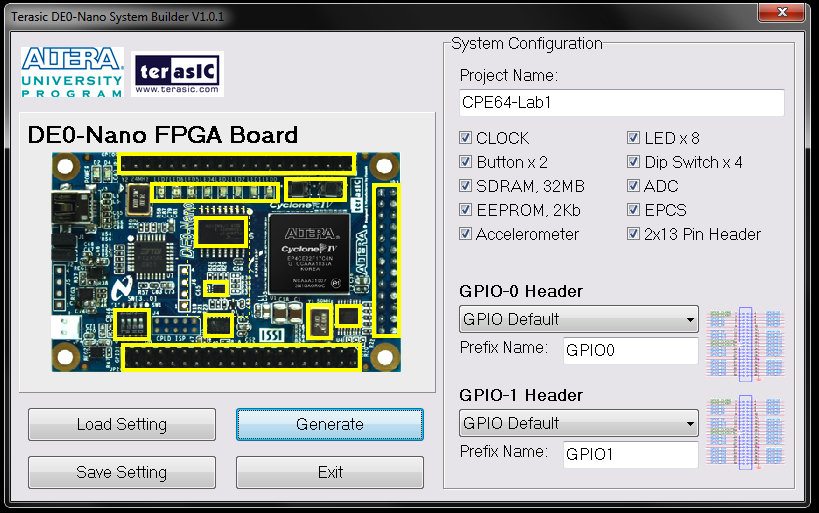
\includegraphics[width=.48\textwidth]{Images/screenshot_88.jpg}
      \caption{TerasIC System Builder GUI}
    \end{figure}
    
    \subsection{Run testbench}
    Now we want to verify our design. Using a simulator for a single logic gate is a bit asinine but
    the experience gained with the test bench will help you greatly in the future. Start a new simulation 
    and add the waveforms as shown in screencast 2. You'll want to have have truth tables laid out for the
    gates your testing so you can be sure they behave the way you expect. Have an extra column ready to record
    the behavior of the FPGA once it's programed.
    
    \subsection{Prepare circuit to test Verilog gate modules with DEO-Nano}
      A switch and LED are going to be used to test the FPGA while it's operating. The LED circuit needs a
      current limiting resistor as shown in the schematic below.
      \begin{figure}[H]
        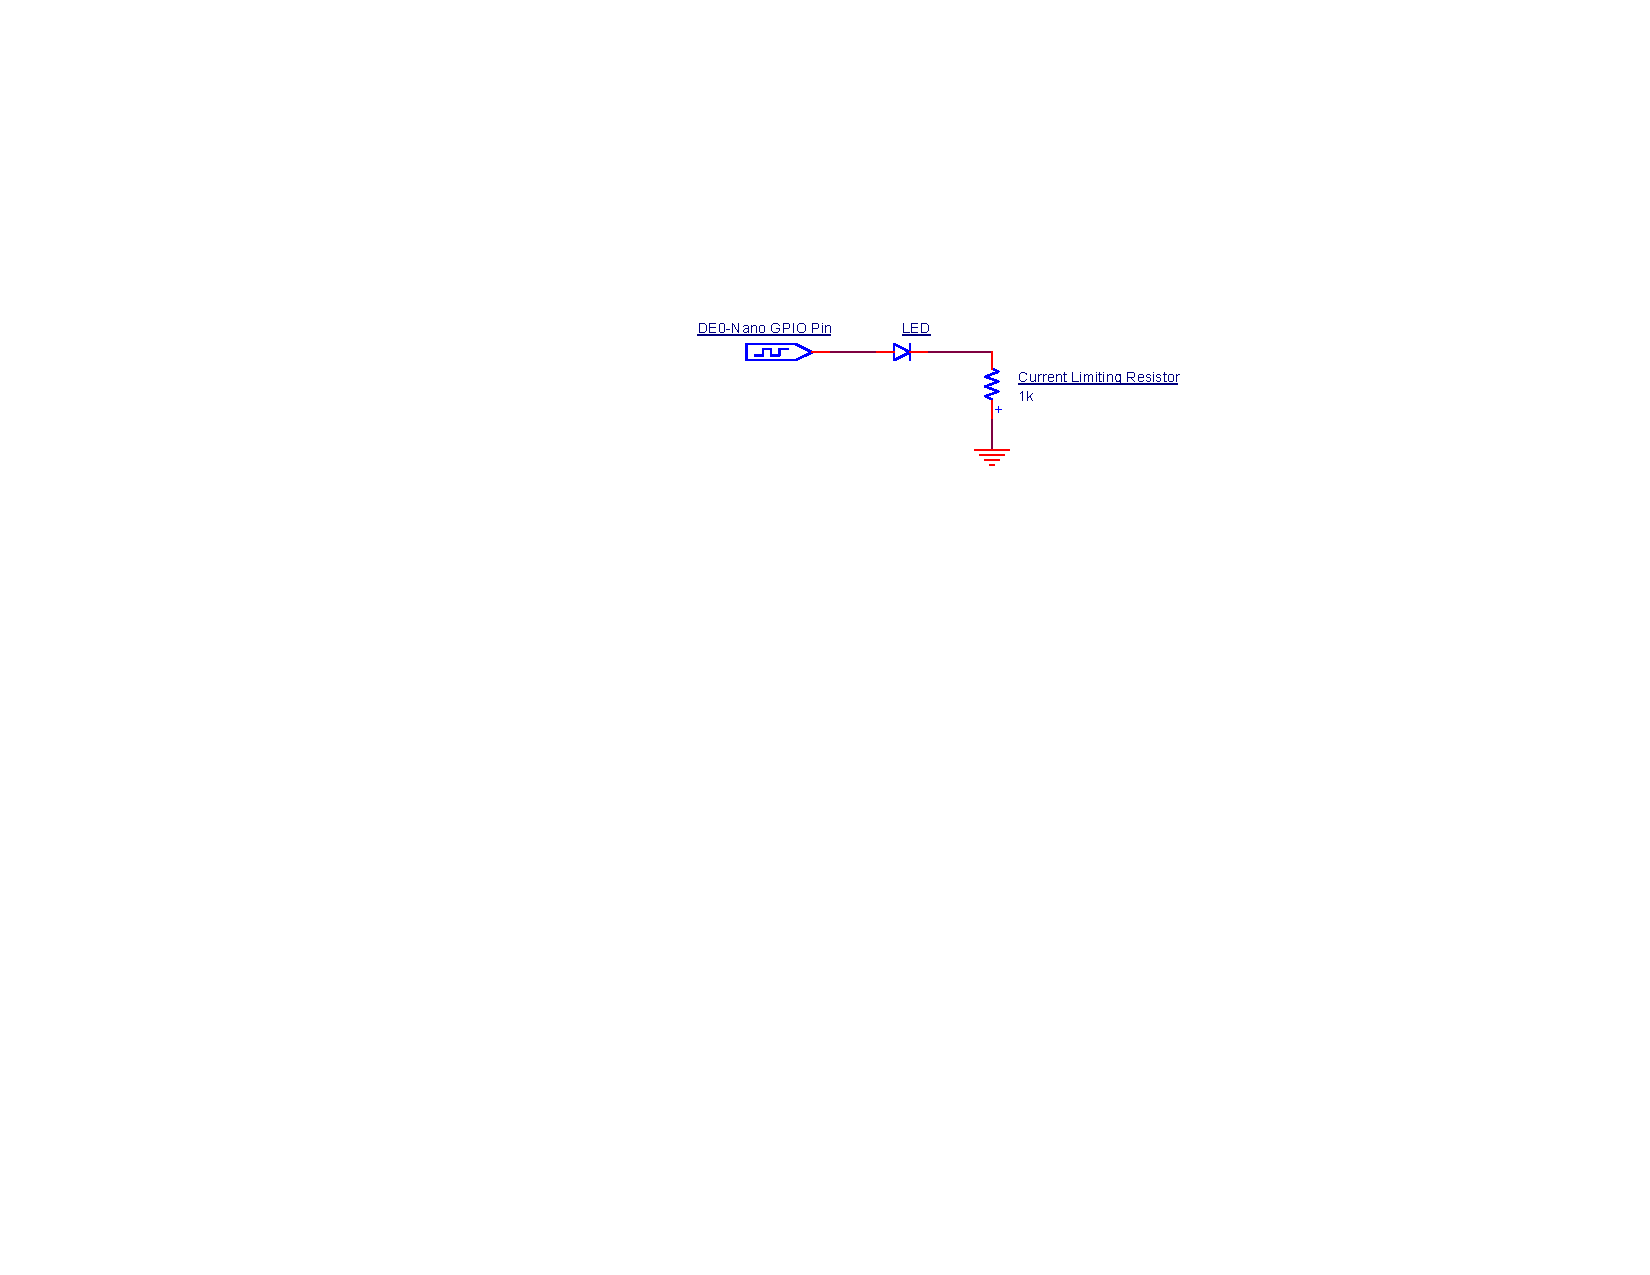
\includegraphics[width=.48\textwidth]{Schematics/LED.pdf}
        \caption{LED with current limiting resistor}
      \end{figure}
      The LED will allow you to see the the output but we'll also need to be able to generate some input for
      the FPGA. We will do this with a dip switch and pulldown resistor. \footnote{The pulldown resistor is needed
      to literally pull the voltage on the pin to ground. Otherwise the pin would switch between 1 and 0 arbitrarily}
      \begin{figure}[H]
        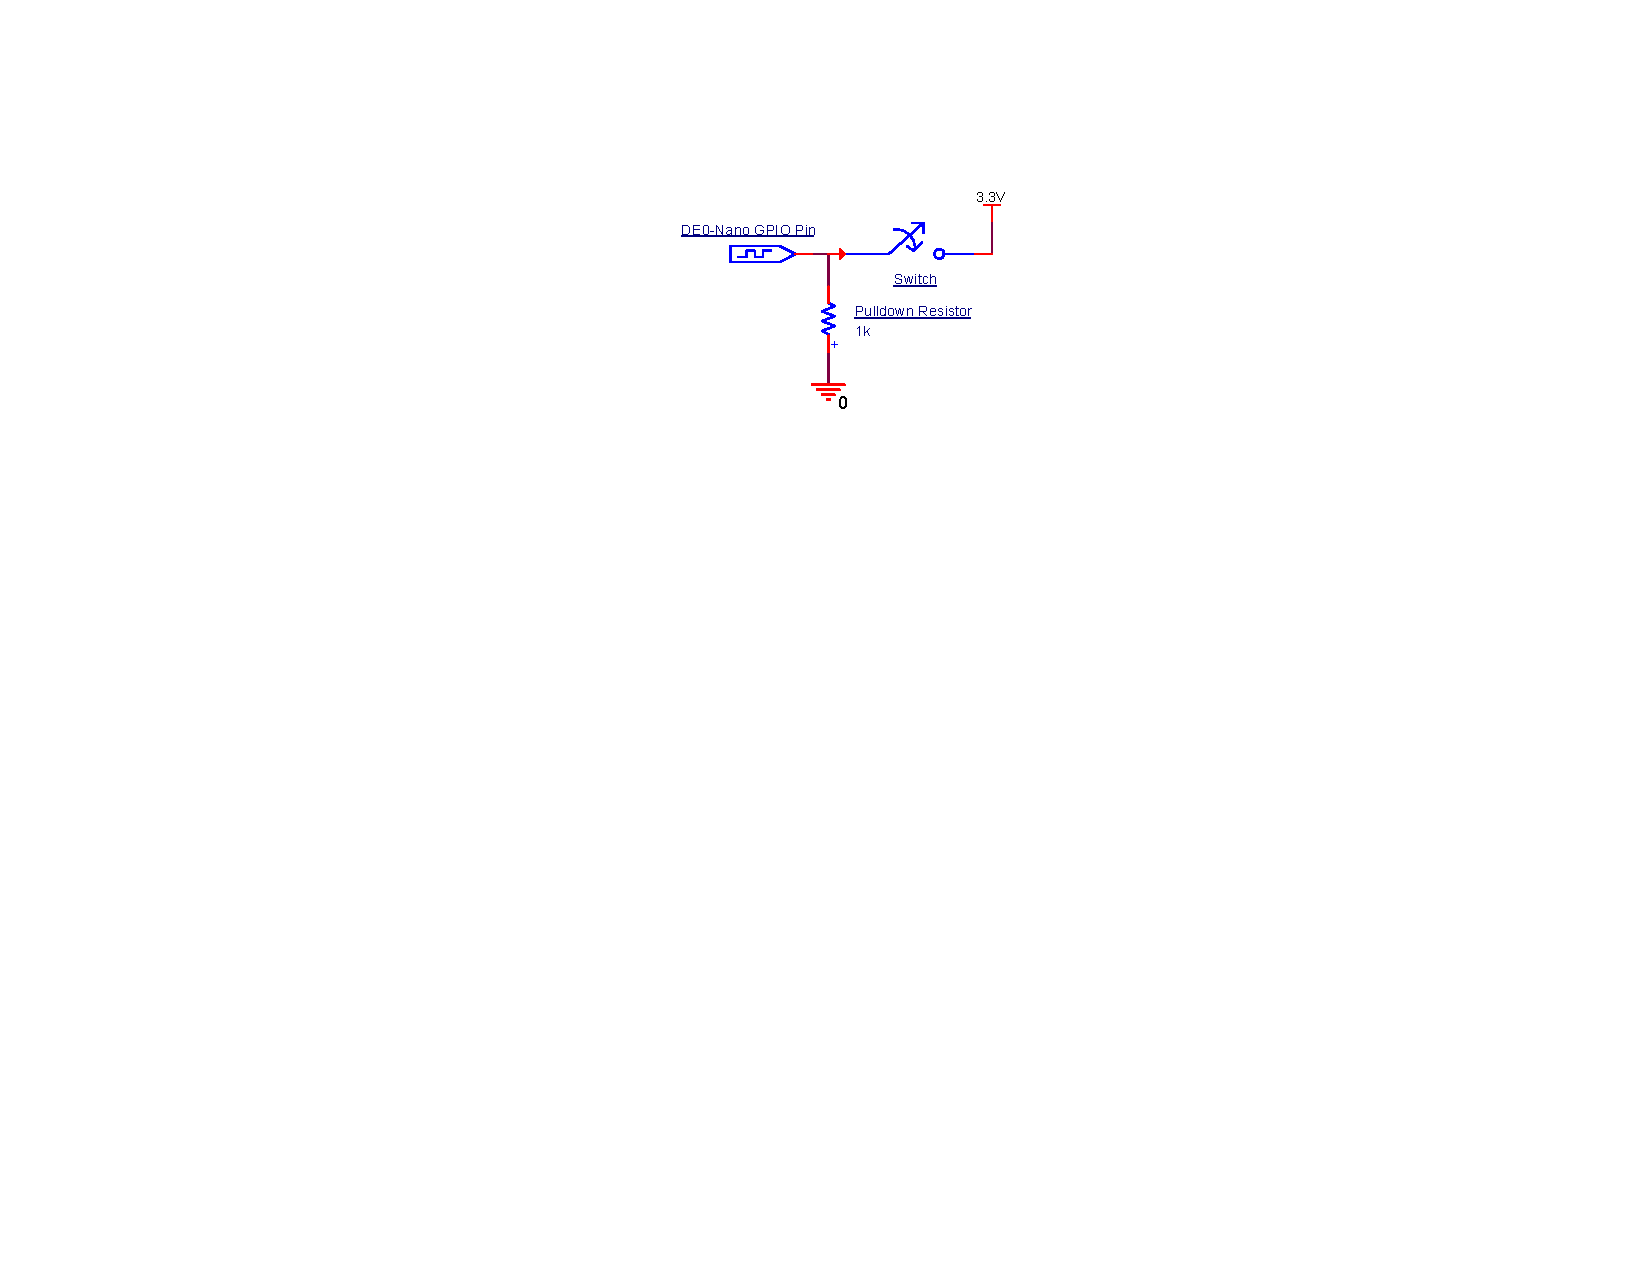
\includegraphics[width=.48\textwidth]{Schematics/SwitchCircuit.pdf}
        \caption{Switch with pulldown resistor}
      \end{figure}

      \begin{figure}[H]
        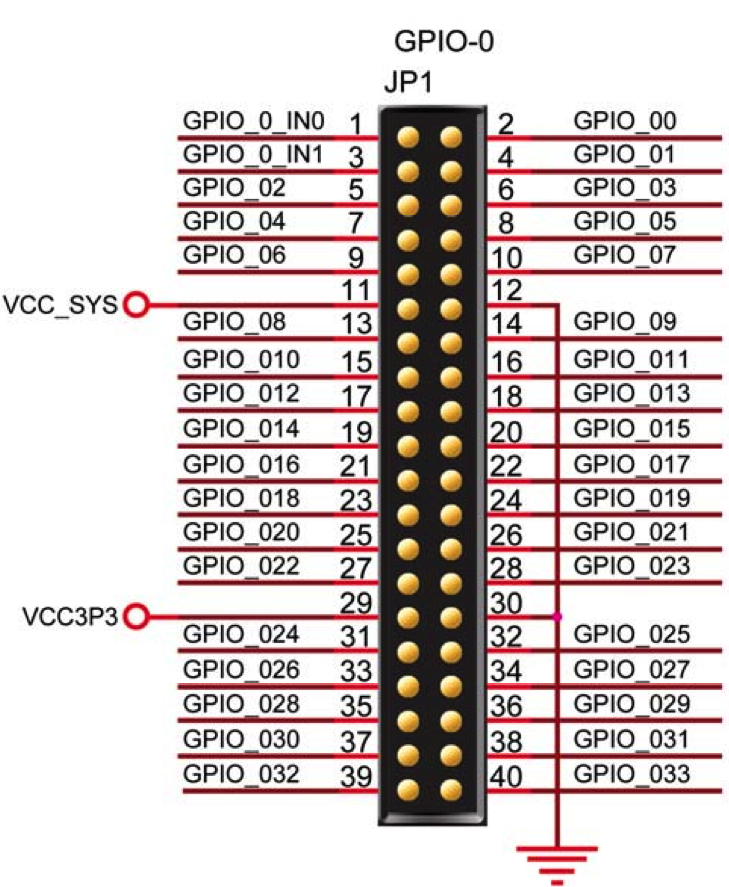
\includegraphics[width=.48\textwidth]{Images/GPIOHeader.jpg}
        \caption{Schematic of GPIO-0 header\cite{DE0Manual}}
      \end{figure}

      \begin{figure}[H]
        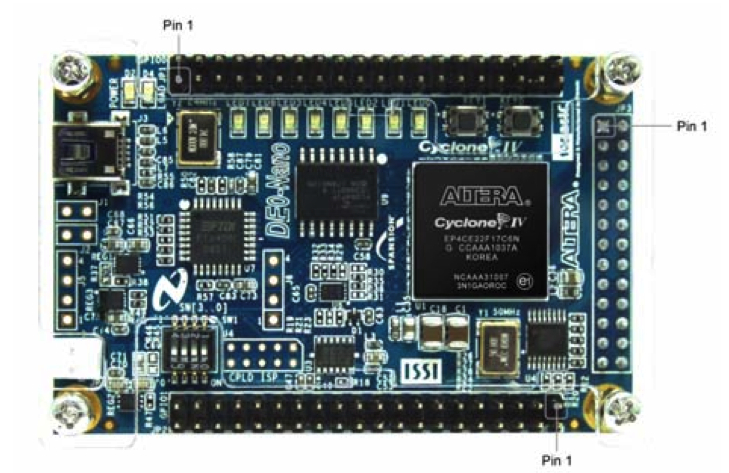
\includegraphics[width=.6\textwidth, angle=270]{Images/LabeledGPIOHeaders.jpg}
        \caption{Orientation of GPIO0 on DE0-Nano development board\cite{DE0Manual}}
      \end{figure}

      \begin{figure}[H]
        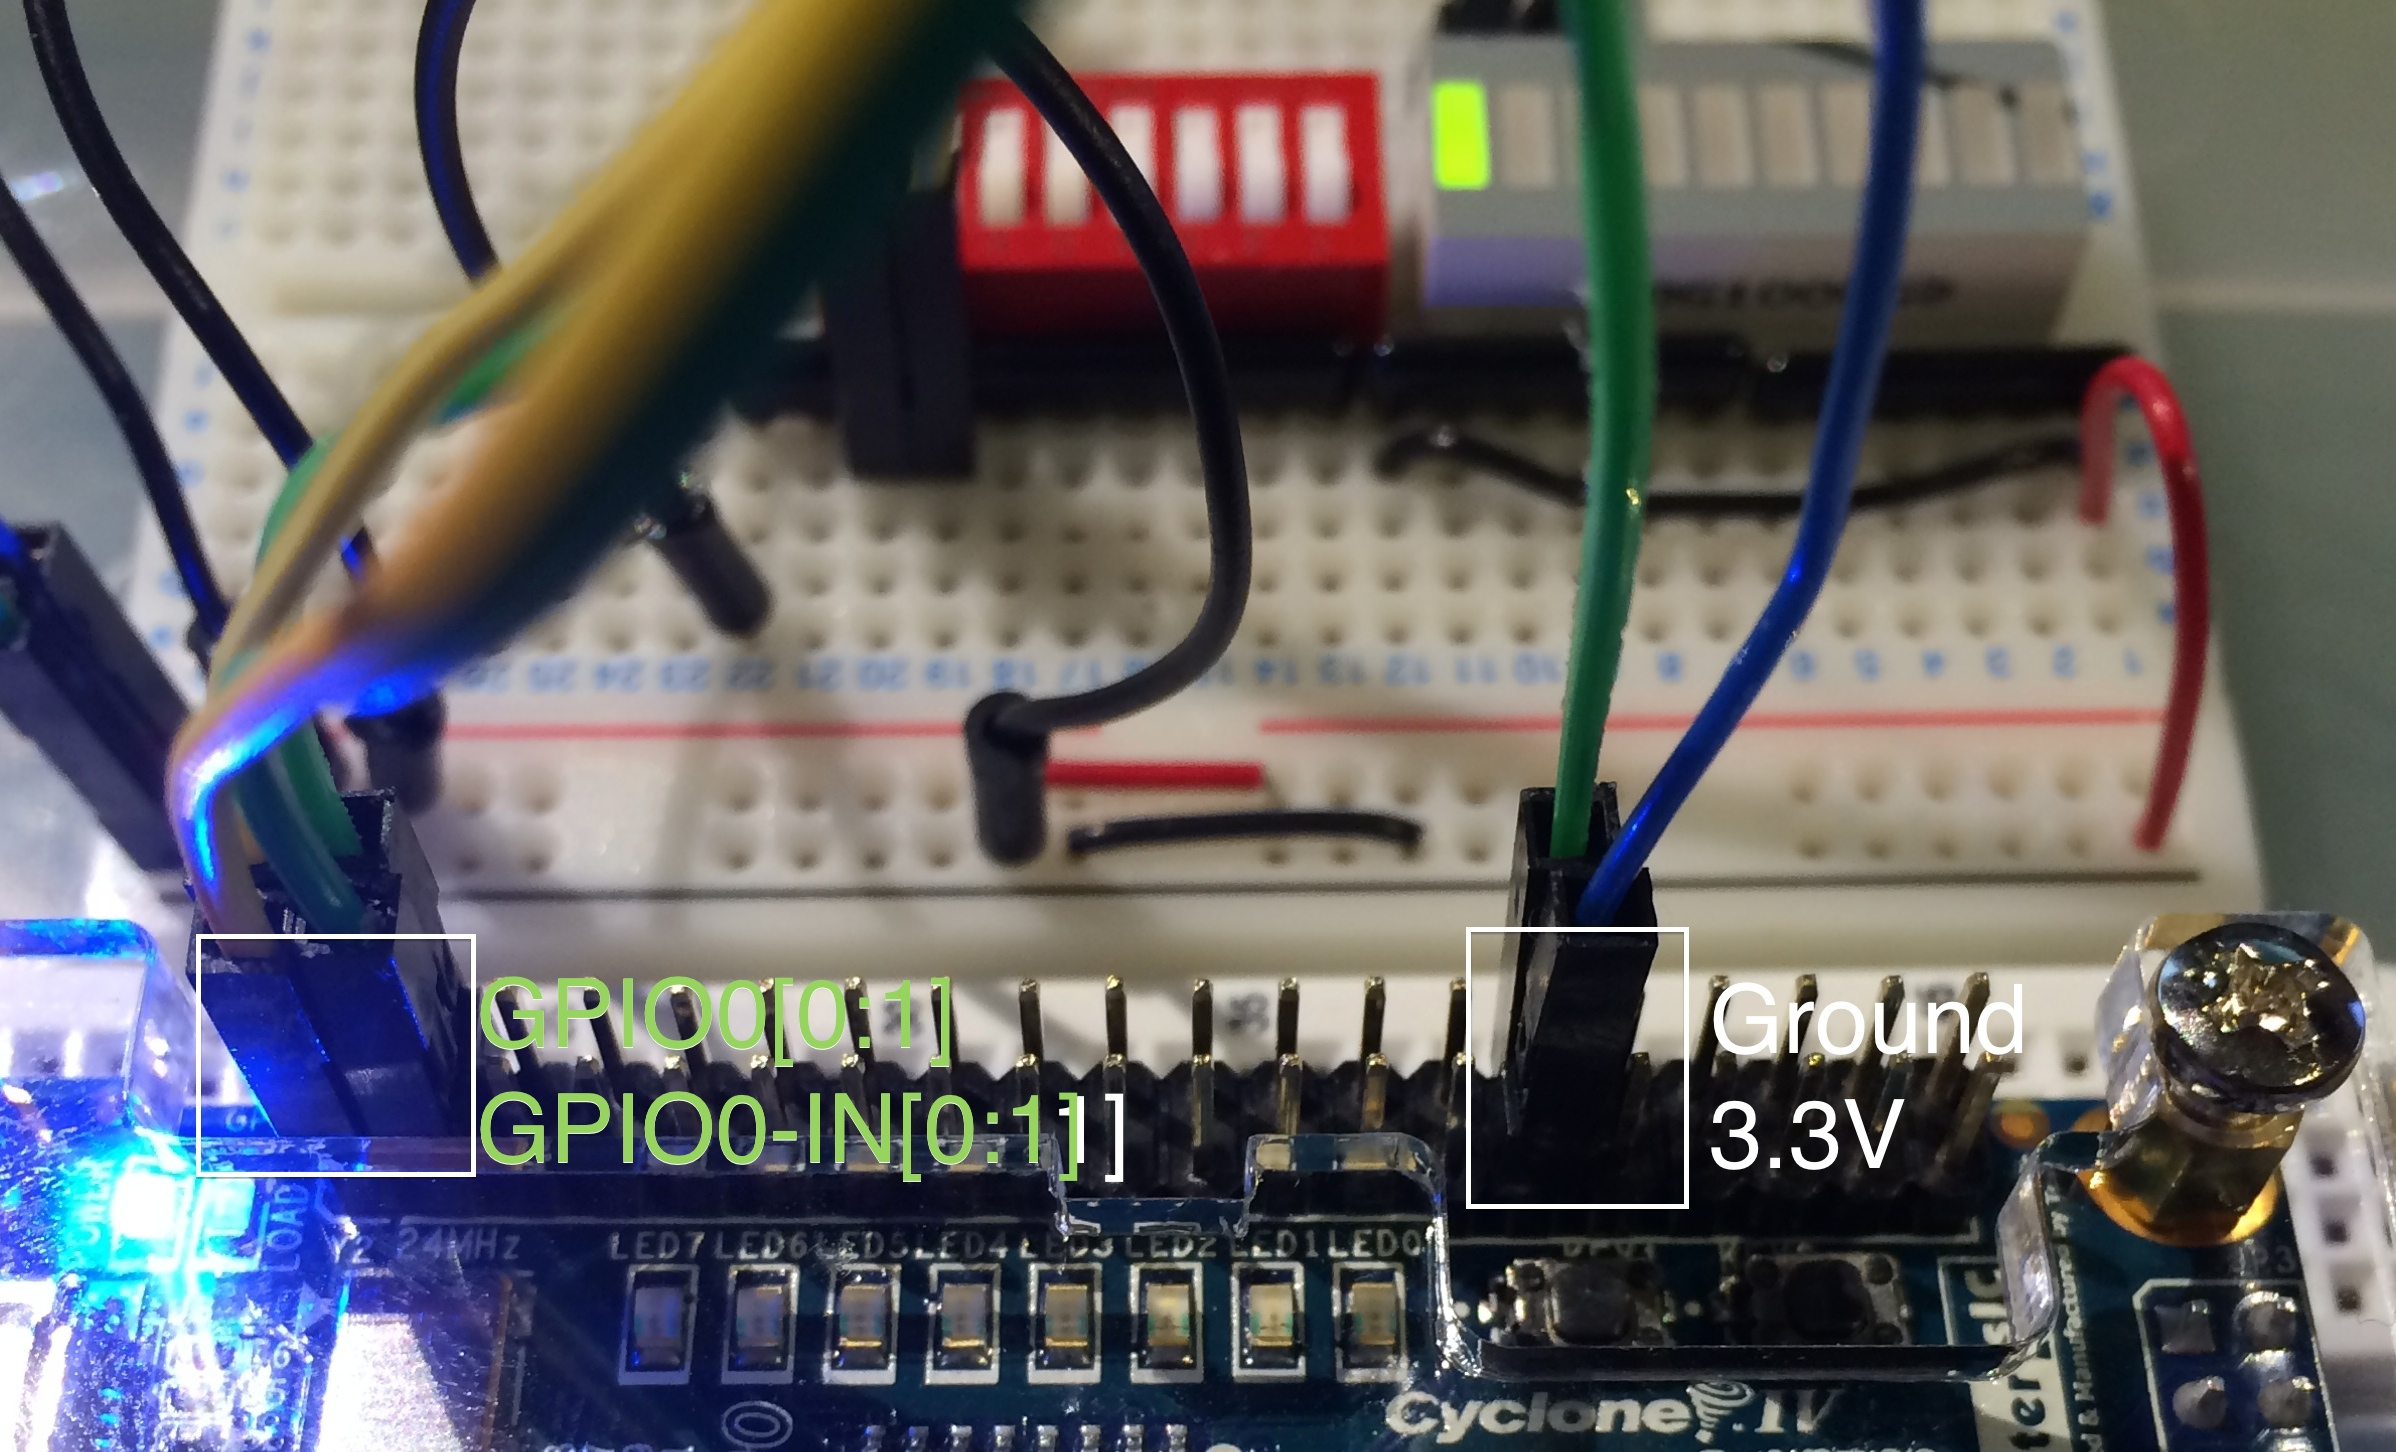
\includegraphics[width=.48\textwidth]{Images/GPIOpicture.jpg}
        \caption{Picture of loaded GPIO-0 header}
      \end{figure}

      \begin{figure}[H]
        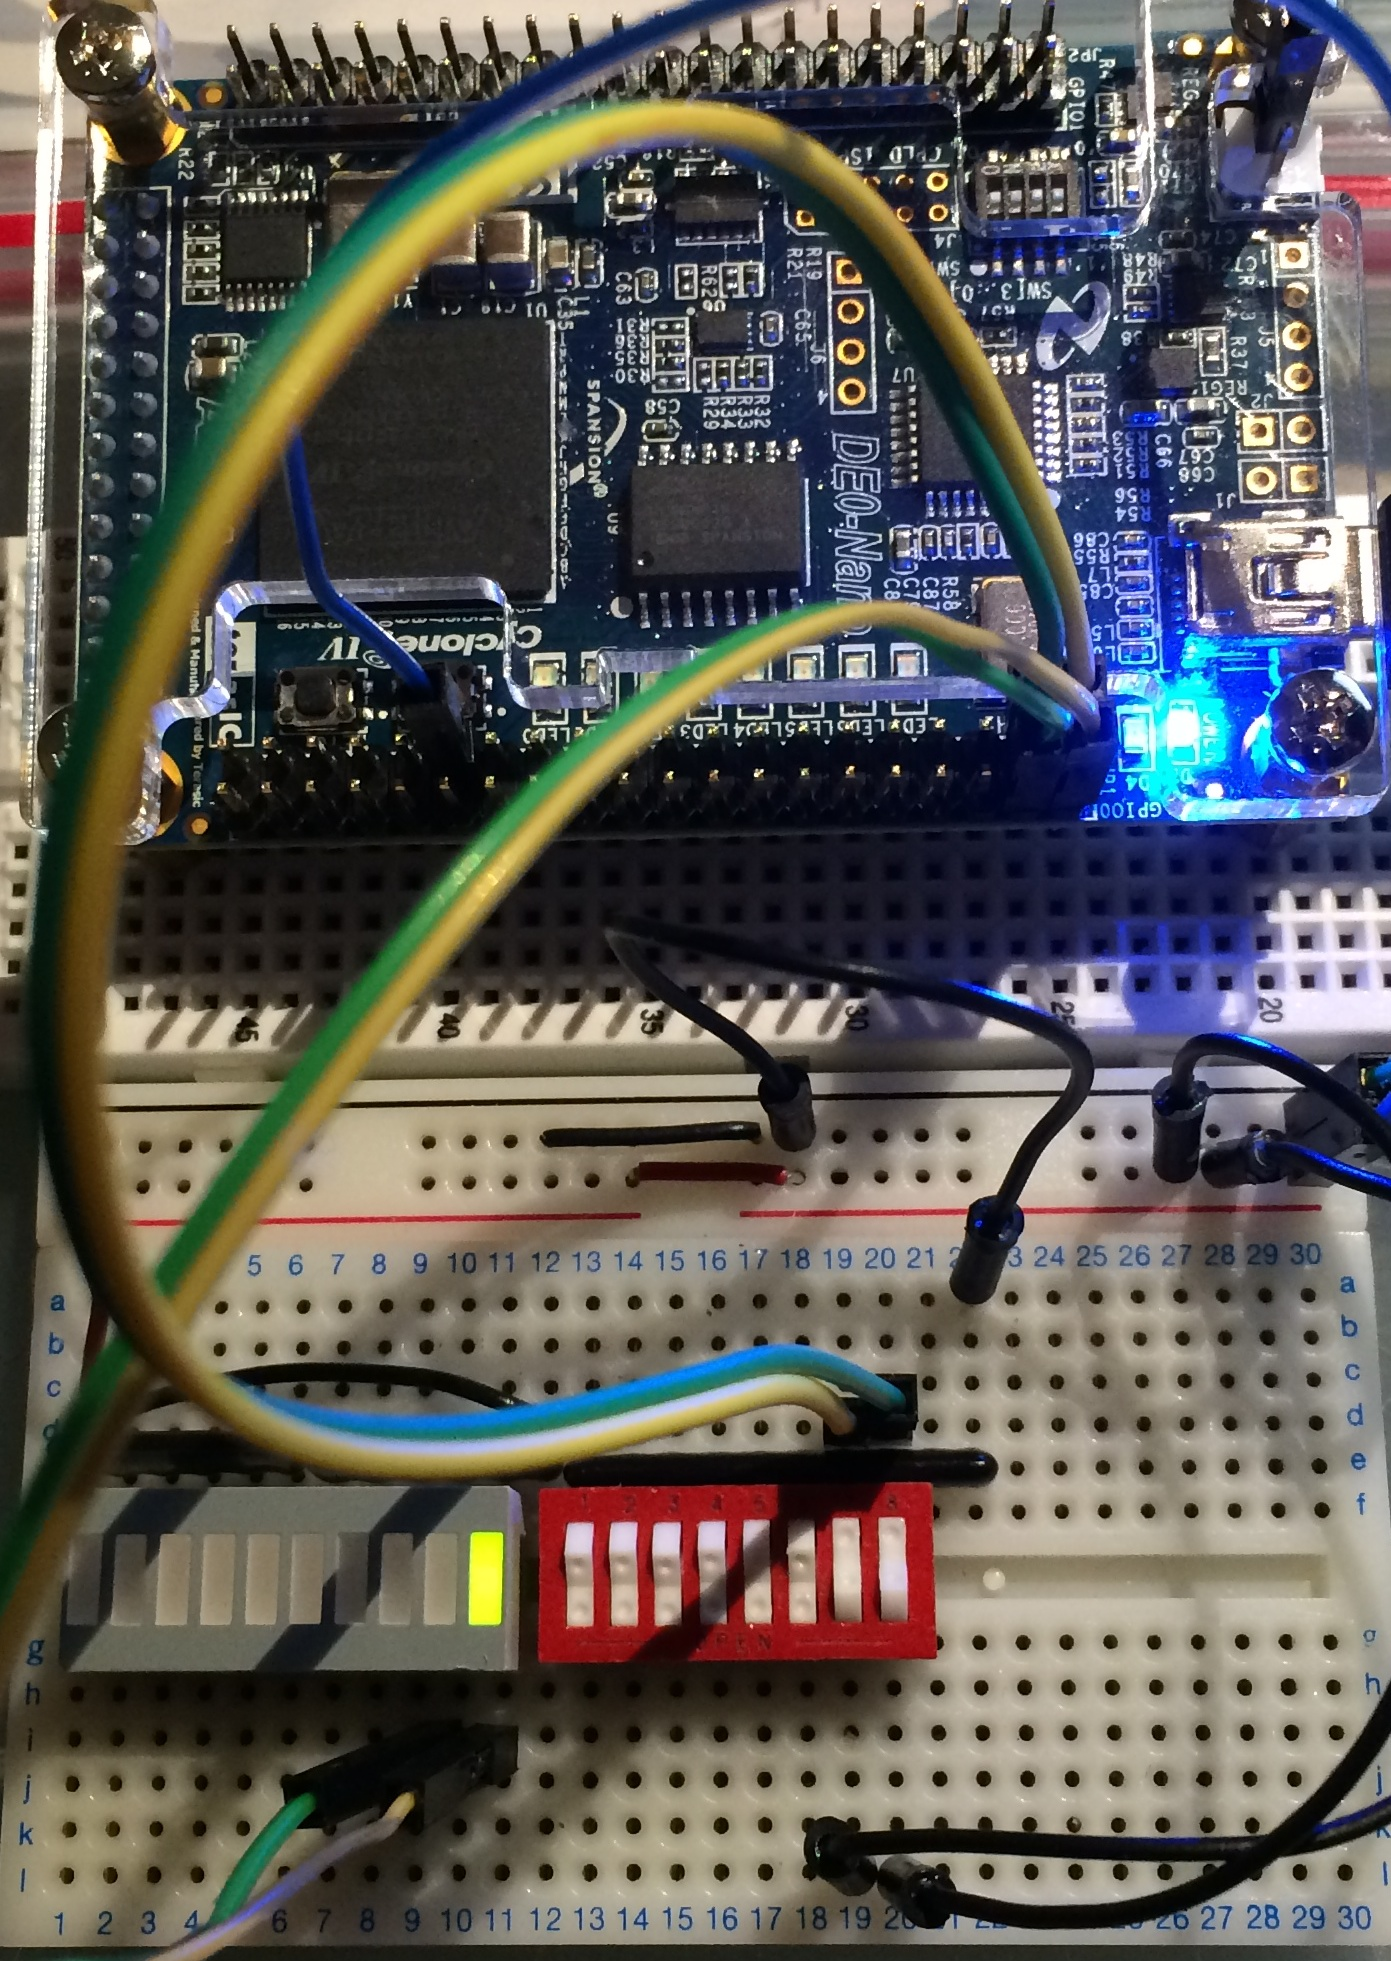
\includegraphics[width=.48\textwidth]{Images/ExampleLayout.jpg}
        \caption{Example switch and LED configuration with SIP resistors}
      \end{figure}

      \subsubsection{Compile example code with Quartus}
        Once you've created and tested your switch circuit we'll need  

      \subsubsection{Use Quartus to program the Nano} refer to screencast 2 for a walk through. After synthesis
      Quartus will generate a .SOF\footnote{the .SOF stands for SRAM object file. This is an Altera standard for
      of their FPGAs.} file that can be used to program the FPGA using Quartus' programmer.
        
      \subsubsection{Test behavior against expected truth table} Use your table from the simulation 

  %| =================================================================================================
  %| Lab Report Requirements
  %| =================================================================================================
  \section{\bfseries  Lab Report}
    The lab report must be typed and submitted in a PDF format. Look to IEEE's guidelines for formatting guidelines
    on format. The document should include
    \subsection{Figures to include}
    \begin{itemize}
      \item Waveform captures from Signaltap and Modelsim
      \item Logic tables from theoretical prediction and experimental outcome
      \item Explanation and listing of your Verilog module.
    \end{itemize}

    \subsection{Questions to answer}
    \begin{itemize}
      \item There are multiple ways to instantiate a module what are three different ways that you could
            instantiate the AND module included with this lab?
      \item Compiling a programming language like C and synthesizing Verilog are very different even though they
            appear to be the same in the IDE. How might 
      \item Notice the report that popss up when you compile your project. There are a number of statistics given
            by Quartus, the logic element usage ratio is your designs use of the total device capacity. More Verilog
            roughly translates into more LC usage. What was your designs Logic Cell utilization. 
    \end{itemize}

  %| =================================================================================================
  %| Conclusions
  %| =================================================================================================
  \section{\bfseries  Conclusion}
    Verilog is an IEEE standard(1364)\cite{Wikipedia:Verilog}, it is pervasive in industry and can be used to develop specialized hardware
    in the form of ASICs or reconfigurable FPGAs. It is important to underscore the differences between Verilog
    and a programming language like C, Java, even Assembly. Verilog offers the ability to take parallel action.
    Two numbers can be multiplied at once, multiple registers can be set and cleared. Entire microprocessors can
    be implemented on the Nano, one of the later labs will explore Altera's softprocessor the NIOS II. The TerASIC
    documentation included with the DEO-Nano kit is pretty good and worth the read. It will help you get the most
    out of the FPGA. The CD included with the Nano will also include circuit schematics that can provide a great
    reference when it comes time to make one of your own.
    \paragraph{More Information} just like anything else the Internet has an amazing amount of information available
    on the Internet to the interested student. 
      \begin{itemize}
        \item \href{http://www.altera.com/education/training/curriculum/fpga/trn-fpga.html}{Altera Traning Curriculum for FPGA designers}
        \item \href{www.eevblog.com}{EEV Blog: What is a FPGA?}
      \end{itemize}

  %| =================================================================================================
  %| Bibliography
  %| =================================================================================================
  \bibliographystyle{IEEEtran}
  \bibliography{IEEEfull}
\end{document}